\section{Introduction}

Hardware system verification has been developed over a large amount of
years, but mostly with limited approaches. Most of works employed
model checking to verify their target system, from processor
verification~\cite{ProcVerif1, ProcVerif2} to cluster
verification~\cite{ClusterVerif}. In order to use model checking
technique, one must first finitize the state-space for exhaustive
exploration, which inherently hinders generalization. Then what should
be defined and developed if one desires to verify highly parametrized
hardware system, such as complex pipelined processors or multi-level
cache-coherence protocols?

Defining formal hardware semantics is the very first step to answer
such question. In model checking it is not required to define
semantics for general hardware system, since checkers have their own
specific targets. However, in order to deal with all aspects of
hardware system, one should be able to define semantics which can
describe all system behaviors. Finally, when formal semantics and
proofs are correctly attached to Hardware Description Languages
(HDLs), it can be claimed that real hardware components are verified.

Now the focus is moved to semantics design: what is good semantics for
hardware system? First of all it should be intuitively understandable,
which implies that the semantics should logically simulate system
behaviors. Moreover, if it is employed for formal proofs, it should
also be in harmony with various proof aspects.

In this proposal, I propose to introduce a number of hardware
semantics, and to compare their pros and cons for better
understanding. I also propose to give formal consistency proofs for
those semantics, which guarantee that the semantics are convertible to
each other. All definitions and proofs will be formally given using
Coq theorem-proving system.

\section{Background: Guarded Atomic Action}\label{sec:background}
Traditional Register-Transfer Level (RTL) designs require hardware
designers to consider scheduling for all resources. During hardware
design, one has to ensure that any resource elements are correctly
employed, e.g., one should not write a register more than once in a
same cycle, which causes incorrect assignment. If a particular input
port of a hardware component is used more than once, we do not have
any guarantees for the output value, also causing incorrect use of
values. A well-known RTL design framework, Verilog, let users take
responsibility of this, thus one should carefully investigate if there
is an assignment which makes incorrect state transition.
%% This low-level approach, however, gives user a chance to directly
%% determine which values should be written in a cycle, therefore to
%% build a well-optimized hardware.
\begin{figure}[h]
  \centering
  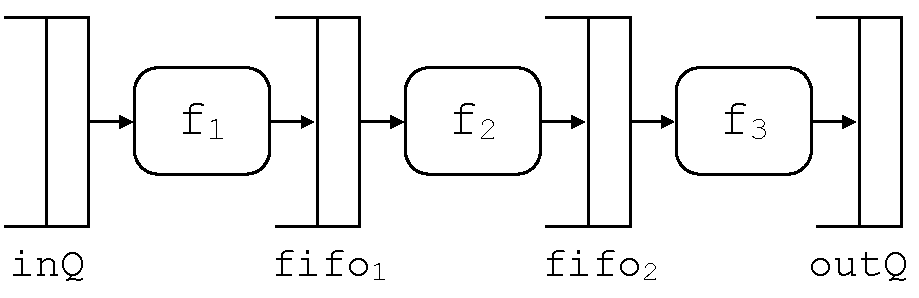
\includegraphics[width=0.5\textwidth]{figures/pipeline.pdf}
  \caption{A pipelined system}
  \label{fig:pipeline}
\end{figure}

A disadvantage of this approach is that having no separation between
functional parts and scheduling logic makes maintenance
harder. Consider a pipelined system where three systems $f_1$, $f_2$,
and $f_3$ are connected by fifos, as shown in
Fig.~\ref{fig:pipeline}. For simplicity, suppose that only one element
can reside in a fifo. Since there is only one element in a fifo, push
and pop cannot be requested in a same cycle -- it will cause
double-write. Now the problem occurs because we have no information
whether push and pop will be requested simultaneously or not. Thus in
this case, we cannot avoid an implementation tightly coupled with
scheduling logic; for each case of push and pop, there is no way for
user but to define different implementations. The design process
entangled with scheduling logic also makes verification harder. We
first have more cases to verify, as there will be different functional
parts as much as scheduling cases. We also have to determine whether
it is caused by funcaional parts or scheduling logic if there is an
error.

Guarded atomic action is a design paradigm for correct and effective
scheduling as well as making up shortcomings of the RTL designs. It is
different from the traditional RTL designs mentioned above. The main
idea is that any hardware system has a (structural) state component
that can be captured by a set of variables that represent registers or
storage. State transition is done by a set of rules, where a rule is a
series of actions on this state. These actions should be atomic -- an
execution of an action should be guaranteed to make a state transition
purely caused by the action.
%% An atomic action induce a guard, a predicate to execute the
%% action. Guards are interpreted by a scheduler to generate a correct
%% schedule, which will be explained in the next section.

\section{Research Questions}

\subsection{Hardware Description Syntax}

\newcommand{\Mod}{\ensuremath{M}}
\newcommand{\ModC}[3]{\ensuremath{(#1, #2, #3)}}
\newcommand{\ModP}{\ensuremath{+}}
\newcommand{\Sem}[1]{\ensuremath{\llbracket #1 \rrbracket}}

Before defining various hardware semantics, we first define a hardware
description language syntax, which will act as a common basis for
defining semantics. First, a basic module $\Mod{} =
\ModC{s}{\vec{r}}{\vec{m}}$ is composed of (internal) state $s$, rules
$\vec{r}$, and methods $\vec{m}$. Each rule or method is a series of
actions, explained in Section~\ref{sec:background}, which only affects
the internal state. Rules are fired by a scheduler which controls the
entire system. Methods can be called by some other modules. Once
modules are defined, we can combine two modules to build a combined
module, using \ModP{} operator. Following is the inductive definition
of a module:

$$\begin{array}{rcl}
  \Mod{} & := & \ModC{s}{\vec{r}}{\vec{m}} \\
  & | & \Mod{} \ModP{} \Mod{} \\
\end{array}$$

One might raise several issues with this syntax definition. For
example, it can be asked whether rule and method names are globally
unique among all modules. This question is interesting in that several
solutions can be given for it. We can globally check whether name
conflict occurs on a module syntax, or we can rather always do
$\alpha$-conversion for all names before two modules are combined.

Once all syntactic issues are resolved, the next step is to give the
meaning of module. It requires to describe the semantics of the basic
module \Sem{\ModC{s}{\vec{r}}{\vec{m}}} and that of \ModP{} operator
\Sem{\ModP{}}. Each semantics should have its own meaning for these
ingredients, which also includes an ability to confirm valid execution
cases and to reject invalid ones.

\subsection{Modular Semantics Inspired by Labeled Transition System}
\label{sec:mod}

Modular semantics regards \Sem{\ModP{}} as a way of
communication. Each basic module has its own semantics by
\Sem{\ModC{s}{\vec{r}}{\vec{m}}}. Now the question is how to describe
the interaction between two basic modules. Such interaction is done by
calling a method. A \emph{label} is defined as a set of method calls,
which implies that method calls are performed between two modules in
an execution cycle. Such concept -- interaction by label -- is based
on Labeled Transition System (LTS), which was originally developed for
communication of concurrent systems.
\begin{figure}[h]
  \centering
  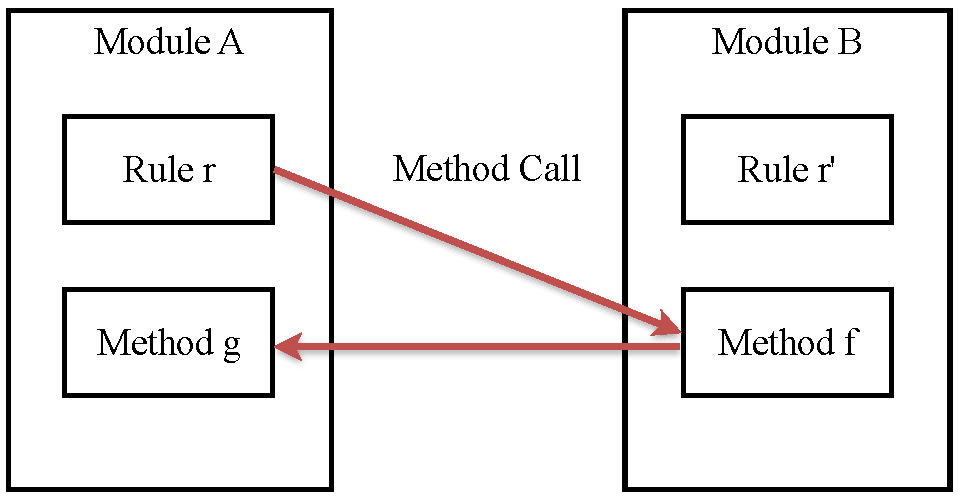
\includegraphics[width=0.5\textwidth]{figures/modular-sem.pdf}
  \caption{Modular Semantics: Interaction by Label}
  \label{fig:mod}
\end{figure}

In modular semantics, \Sem{\ModP{}} as an interaction inherently
involves checking correctness of a label, which might be tedious to
deal with large modules. For example, if two modules $A$ and $B$
communicate by method calls shown in Fig.~\ref{fig:mod}, semantics of
module $A$ should contain execution of rule $r$ and method $g$, and
that of module $B$ should contain execution of method $f$. That is, in
order to deal with \Sem{\ModP{}} on \Sem{M_1 \ModP{} M_2}, we should
be able to deduce entire relevant information from \Sem{M_1} and
\Sem{M_2}. It is quite easy to extract such information if $M_1$ and
$M_2$ are basic modules, but what if they are combined modules? Then
we have to inductively obtain information from them again. From the
perspective of (mechanical) proof, algorithms for deriving such
correctness of labels should be efficiently defined for proof
automation performance. It would be a good research question to study
inherent limitation of modular semantics and to find efficient
algorithms for overcoming it.

\subsection{Inlined Semantics}

Inlined semantics regards \ModP{} as a syntactic (static) inlining
operator. In other words, $\Sem{M_1 \ModP{} M_2} \triangleq
\Sem{M_{12}}$, where $M_{12}$ is a basic module resulted from inlining
between $M_1$ and $M_2$, which are also basic modules. Note that even
if a module is composed of a number of basic modules, it is still
possible to define the semantics inductively, e.g., $\Sem{(M_1 \ModP{}
  M_2) \ModP{} M_3} = \Sem{M_{12} \ModP{} M_3} = \Sem{M_{123}}$.

Inlined semantics has its own advantage in that it is intuitive to
understand, but it lacks modularity. Inlining has been broadly used
for any languages to describe the semantics where a number of
interface calls happen. The concept is quite intuitive -- we
substitute a method call to its body to obtain same effect. However,
once we derive an inlined module on the semantics, we lose information
which can be deduced from the original modules. For example, if one
want to claim two combined modules $M_1 \ModP{} M_2$ and $M_1 \ModP{}
M_3$ are similar to each other, on inlined semantics, one should deal
with inlined modules $M_{12}$ and $M_{13}$ directly. Whereas on
modular semantics described in the previous section, we only need to
say $M_2$ and $M_3$ are similar.

\subsection{Small-step and Deterministic Semantics}

Small-step semantics can be viewed as a dynamic version of the inlined
semantics. Like standard small-step semantics definitions for several
procedural programming languages such as C, a method call is used to
invoke a new execution context for some other modules.  Execution
stack is the most popular concept to deal with small-step semantics
with method calls. On small-step semantics, \ModP{} is merely used to
connect method calls and their bodies.

The core advantage of the small-step semantics is that executions can
be \emph{evaluated} through global module structure, which in turn
hinders modular reasoning. That is, one can define small-step and
\emph{deterministic} semantics for hardware system. Having global
module definition makes it possible -- one should know which other
modules will be affected by each method call. However, to put it the
other way, we cannot give the semantics for a basic module, say
\Sem{M_1} alone on \Sem{M_1 \ModP{} M_2}, since interfaces of $M_2$
should be given.

\subsection{Semantics Consistency}

Once various semantics are defined, we should be able to prove
consistency among semantics. As briefly stated in previous sections,
each semantics has its own pros and cons. However, it does not mean
that a specific semantics should be chosen and thus other semantics'
advantages cannot be gained. It should be possible to convert
semantics whenever we want so that all advantages of the semantics can
be enjoyed. Proving semantics consistency is hence an essential work
for building better environment.

\section{Work Plan}

Currently we have a firm basis for modular semantics~\cite{CAV},
described in Section~\ref{sec:mod}. We have designed and implemented
the semantics using Coq theorem proving system. The semantics has been
actively used to prove non-trivial facts of hardware
systems. Therefore it should be enough to claim valid arguments that
when the modular semantics is strong and when is not.

On the other hand, inlined semantics and small-step semantics should
be formally defined, which is the very first step to do now. Currently
I am defining formal inlining functions by Coq with some correctness
proofs. I hope these semantics will be defined by the end of
January. In addition to the semantics definitions, consistency proof
should be given, which would be one of final goals of the project. I
expect a month is enough to finish the proof, thus all things should
be done by the end of March.

Finally, I will be spending $1.5$ -- $2$ months to write my thesis.
Following is the briefly organized plan for my master thesis:

\begin{figure}[h]
  \begin{center}
    \begin{tabular}{l|l}
      \hline
      Month & Plan \\
      \hline
      Nov, 2015 -- Dec, 2015 & Define inlined semantics and prove its correctness \\
      Jan, 2016 -- Feb, 2016 & Define small-step semantics \\
      Mar, 2016 & Prove consistencies among semantics \\
      Apr, 2016 -- May, 2016 & Write the thesis \\
      \hline
    \end{tabular}
  \end{center}
\end{figure}
